\documentclass{article}

\usepackage[english]{babel}
\usepackage[letterpaper,top=2.5cm,bottom=2.5cm,left=2.5cm,right=2.5cm,marginparwidth=1.75cm]{geometry}
\usepackage{amsmath, graphicx, tikz, pgfplots, multirow, newlfont, gensymb, indentfirst, bm, setspace, fancyhdr, pdfpages, xurl, pdflscape}
\usepackage[export]{adjustbox}
\pagestyle{fancy}
\fancyhf{}
\rhead{Group 2 \\ 12/7/22}
\lhead{CE-321\\Structural Engineering}
\cfoot{\thepage}
\renewcommand{\headrulewidth}{1.5pt}
\setlength{\headheight}{22.6pt}
\usepackage[colorlinks=true, allcolors=black]{hyperref}
\setlength\parindent{24pt}
\pgfplotsset{scaled y ticks=false}
\pgfplotsset{scaled x ticks=false}
\pgfplotsset{width=12cm, compat=1.18}

\begin{document}
    \begin{titlepage}
    \begin{center}
    {{\Large{\textsc{The Cooper Union for the Advancement of Science and Art}}}} \rule[0.1cm]{15.8cm}{0.1mm}
    \rule[0.5cm]{15.8cm}{0.6mm}
    {\small{\bf DEPARTMENT OF CIVIL AND ENVIRONMENTAL ENGINEERING}}\\
    {\footnotesize{STRUCTURAL ENGINEERING LABORATORY}}
    \end{center}
    \vspace{15mm}
    \begin{center}
    {\large{\bf LAB 5\\}}
    \vspace{5mm}
    {\Large{\bf COMPRESSIVE TESTING OF\\}}
    \vspace{2mm}
    {\Large{\bf STANDARD CONCRETE CYLINDER}}
    \end{center}
    \vspace{35mm}
    \par
    \noindent
    \hfill
    \vspace{20mm}
    \begin{center}
    {\large{ {\bf Group 2} \\ { Jenna Manfredi\hspace{5mm}David Madrigal\hspace{5mm}Gila Rosenzweig\\Nicole Shamayev\hspace{5mm}Jake Sigman}}}
    \vspace{40mm}
    {\large {\bf \\CE-321 \\ 12/14/22 \\}}
    \vspace{15mm}
    {\normalsize{Professor Tzavelis \\ Avery Kugler \\ Lionel Gilliar-Schoenenberger \\ Crystal Woo}}
    \end{center}
\end{titlepage}
    \doublespacing
    \tableofcontents
    \newpage
    \addcontentsline{toc}{section}{List of Tables}
    \listoftables
    \addcontentsline{toc}{section}{List of Figures}
    \listoffigures
    \newpage
    \section{Objective}
    \indent The purpose of this project is to design a bridge that follows the constraints from the annual AISC/ASCE National Student Steel Bridge Competition rules. These constraints are to design a bridge that yields at a force of 800 lbs when loaded at mid-span using the MTS 793 hydraulic actuator. The bridge dimensions need to be 6 feet in length and have a minimum vertical clearance of 6” at mid span. The unobstructed cross-sectional opening is 6” by 14” to ensure vehicles can pass through the opening. The bridge cannot support more than 1000 lbs as this would mean it is overdesigned. It also cannot have members longer than 30”. The group is responsible for carrying out an original design that involves decisions on connections and member dimensions keeping in mind the material, overall bridge shape, and aesthetics. The group develops skills in 3D modeling, calculating for design, cutting members, and welding for this project. The experiment is conducted in the Civil Engineering Structures Lab at the Cooper Union (room LL220).
    
    \newpage
    \section{Procedure}
    \subsection{Design}
    \indent The first part of the process is for all group members to come up with a tentative wire-frame bridge design in AutoCAD. During class, group members are tasked to determine the most optimal structure for fabrication. Our group decided on a mix of two group member's designs since they didn't include any arches or overbearing complexities. We ultimately ended up simplifying even more since the proposed designs would be too busy for a six-foot bridge. After coming to a consensus about the aesthetics of the bridge, the next step is to put the model into Robot Structural Analysis Professional software. The model is entered as a 3-D truss with the appropriate loads. The bridge geometry is further optimized based on the analysis results from Robot. Low force members are removed and the appropriate zero-force members are implemented. Based on the analysis, calculations are performed to determine material, member cross-section, member width and the appropriate material costs. Design members are also designed using a safety factor of 1 where the bridge should yield if the designated load is applied in the middle. The cross-sectional area of the members are calculated using stress and an applied force of 1000 lbs since this is the force that cannot be exceeded by the bridge. We ultimately decided on round members since the square members available did not meet our calculated cross-sectional calculations. Since our members are small and rounded, we also decided to weld our bridge connections. Connections are made with a safety factor of 2.
    \subsection{Fabrication}
    \indent To map out the dimensions, necessary cuts, and welds for the members a full-scale CAD of the bridge is printed. This construction drawing is useful when keeping track whether the members are adequately cut and how many have been cut so far. Once the shipment of steel arrived, the members were cut. After putting on protective eye gear, each steel rod with a smaller cross-section is first fixed to a table using C-clamps with the end sticking out about two inches longer than the planned cutting length. Then, the rod is measured and marked with a sharpie where the saw will be. Cutting with the saw creates a tolerance which needs to be accounted for by cutting slightly longer than the planned dimension. For steel with larger cross-sections, a drop-saw is used. The member is placed in the machine, then a mechanical saw controlled by a motor drops very slowly over the member, allowing for precise cuts for thicker members. After each member is cut, it is taken to a disk sander to be de-burred, a process that involves the removal any uneven edges from sawing. Members that need angled cuts are beveled accordingly. This process is repeated for all members. \\
    \indent To weld the bridge, Tungsten Insert Gas (TIG) Welding is used. The steel is cleaned first, so that any coatings do not react with the gas from the welding machine. Since each member is de-burred and beveled there is a groove between members for the weld to sit in, and effectively join the members. When welding, the proper protective gear is put on, including a welding helmet to filter out the bright radiation from the welding spark. Because the members of the bridge are very thin, the pedal must be pressed carefully to commence the weld. The amount gas being released by the machine is also lowered. When welding, a pool of melted steel forms on the surface of the metal before adding in the steel welding rod that forms tack welds. This process was used along the entire bridge, using angles and clamps to hold the bridge in the correct shape while welding. Once the whole bridge is tacked in place, every weld is repeated, adding more steel welding rod to fill in any holes, and to ensure that the connections are complete and solid welds. 
    \subsection{Testing}
    \indent The fully fabricated bridge is tested using an MTS 793 Hydraulic Actuator. The bridge was supported by steel weights placed at the four corners along the bottom chords and loaded with a 1' by 1' steel plate on the tip of the bridge. The bridge buckled at 770.5 lbs meeting the minimum load requirement of the project. 
    \newpage
    \section{Theory}
    \noindent A truss is defined to be a structure composed of slender members joined at their endpoints; all loads are applied at the joints, and therefore  members of the truss will only develop an axial force under loading. The joints are assumed to be connected as smooth pins, even if there is some rigidity from fabrication. Any bending stress developed during the fabrication of a truss is defined as \emph{secondary stress}. The axial stress developed from loading is defined as \emph{primary stress}. In this laboratory project, only primary stresses are considered in both the hand calculations and the finite element analysis software.
    \\\\
    Members experiencing tensile loads in the elastic region of the material follow Hooke's Law: 
    \begin{equation}
        \sigma = E \varepsilon 
    \end{equation}
    Where $\sigma$ is the applied stress, \emph{E} is the \emph{modulus of elasticity} of the material, and $\varepsilon$ is the strain. 
    Under loading, members will experience a deflection $\delta$; the percent change in the original length $L$ of the member is defined as the strain $\epsilon$. 
        \begin{equation}
            \epsilon = \frac{\delta}{L}
        \end{equation}
    Materials undergoing loading will exhibit elastic deformation when Hooke's Law holds; different materials will experience higher or lower deflections depending on their modulus of elasticity.
    \\\\Hooke's Law holds true for compression loads as well; however, equation 1 fails to consider the stability of the member in question. Specifically, compression members undergo \emph{buckling}, which is the phenomenon observed as the shape change of a member. A compression member with length \emph{L} will buckle at the critical load $P_{cr}$ as governed by the following equation: 
    \begin{equation}
        P_{cr} = \frac{\pi^2 E I}{(KL)^2} 
    \end{equation}
    where $I$ is the moment of inertia of the cross-section of the column, and $K$ is the \emph{effective length constant}. Equation 3 is defined as \emph{Euler's formula}. Truss members that are slender are especially susceptible to buckling failure and therefore must be either braced somewhere by the center of the member or the member must be designed to be thicker. In considering the eccentricities of the loading, the bridge must be braced laterally in order to prevent instability and lateral-torsional buckling; thus, diagonal bracing such as a K-truss can be used to prevent three-dimensional geometric failure. \\
    Lastly, under a single point loading \emph{zero-force members} can be expected. A zero-force member does not carry any of the developed loads. However, zero-force members are necessary for load variations and bracing, which are to be expected in this project.
    \newpage
    \section{Results}
    \doublespacing
    % Force Deflection Image

    % Sample Calculations - P_crit, Stress, Bridge Score
    \subsection{Cross-Sectional Area Calculation}
    \noindent The first calculation performed to determine the required cross-sectional area was the calculation using stress. The calculation for stress is as follows:
    \[\sigma=\frac{P}{A}\] 
    \noindent Where \(\sigma\) is the yield stress of steel, given as 36,000 pounds per square inch, \(P\) is the applied force, which was targeted at 1000 pounds, and then the cross-sectional area, \(A\), which was to be determined. Rearranging the equation for cross-sectional area, the following equation is given:
    \[A=\frac{P}{\sigma}\] 
    \noindent Substituting for \(P\) and \(\sigma\) gives the following:
    \[A=\frac{1000 \text{ lbs}}{36000\text{ psi}}=\boxed{0.028 \text{ in}^2}\]
    \noindent Once the cross-sectional area was determined, the critical buckling load must be determined to ensure that no vertical members undergo buckling as the bridge is loaded. The equation for critical buckling load is as follows:
    \[P_\text{crit}=\frac{\pi^2\times E\times I}{k\times L^2}\]
    Where \(P_\text{crit}\) is the critical buckling load, \(E\) is the modulus of elasticity of steel, given as 29,000 kilopounds per square inch, \(I\) is the moment of inertia of the cross-section, \(k\) is an adjustment factor, taken as 0.83, and \(L\) is the height of the bridge.
    \[P_\text{crit}=\frac{(\pi^2)\times (29000\times10^3\text{ psi})\times (0.00047\text{ in}^4)}{(0.83)\times (19.69\text{ in})^2}=\boxed{502\text { lb}}\]
    This is the critical buckling load for one side truss. Since the structure contains two side trusses, the critical buckling load is double of the calculated value, exceeding the total 1000-pound force, ensuring that no buckling will occur in each of the side trusses.
    \newpage
    \subsection{Force-Deflection Diagram}
    \noindent Below is the force-deflection diagram as the bridge was loaded:
    \begin{center}
        \addcontentsline{lof}{figure}{Figure 1: Force-Deflection Diagram}
        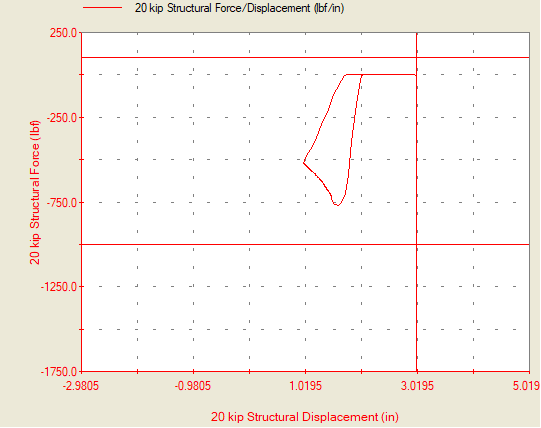
\includegraphics[scale=0.8, frame]{deflection.png}
        \\Figure 1: Force-Deflection Diagram
    \end{center}
    It was found that the maximum force applied to the bridge before the bridge began to yield was \(\boxed{-770.5\text{ lb}}\) and the maximum deflection of the bridge was \(\boxed{0.9805\text{ in}}\)
    \subsection{Bridge Score}
    % Use 10 lbs for Weight, 12 hours for time, 5 for Team Size, $94.48 for Cost, 0.9085 in for Deflection, 5 for Aesthetics
    \noindent The bridge score was calculated using the following equation:
    \[S=(\$5.00 \text{ per pound})\times W+ (\$2.00 \text{ per hour})\times N\times T +(\$300 \text{ per inch})\times\Delta+C+(\$2.00)\times A\]
    Where \(W\), the weight of the bridge, is 10 pounds, \(N\), the build team size, is five, \(T\), the build time, is 12 hours, \(\Delta\), the deflection, is 0.9085 inches, \(C\), the materials cost, is \$94.48, and \(A\), the aesthetics score, is 5.
    \[S=(\$5)\times (10 \text{ lbs})+ (\$2)\times (5)\times (12 \text{ hours}) +(\$300)\times(0.9085\text{ in})+(\$94.48)+(\$2)\times (5)=\boxed{\$547.03}\]
    \newpage
    \section{Lessons}
    \indent During testing, our bridge experiences second-mode buckling. While designing our bridge, to account for buckling, we used a \(k\) value of 0.83. This was because the bridge would be welded, so the ends were not pins, so the \(k\) value should not have been considered equal to 1. However, despite welds being a fixed connection, it was possible that the welds could only be partially all-around welds, and as a result, cannot be considered fully fixed. To account for this, we used a \(k\) factor between 1 and .65, to generate a critical force for somewhere between a fixed and a pinned joint (see figure 2). 
    
    \begin{center}
        \addcontentsline{lof}{figure}{Figure 2: \(k\) Values for Column Buckling}
        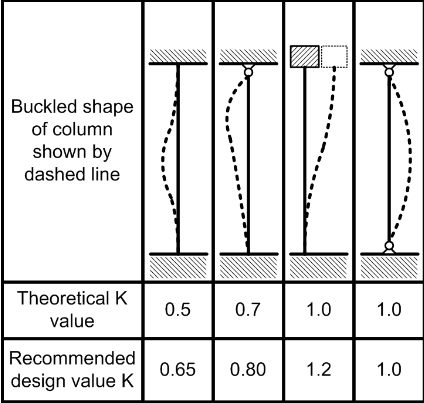
\includegraphics[scale=1, frame]{buckling.png}
        \\Figure 2: \(k\) Values for Column Buckling
    \end{center}
    
    The member along the top chord of the truss experienced a second-mode buckling pattern because of the vertical zero-force member placed in the hypotenuse midpoint. This created a third joint along the member, which allowed for a point of inflection about the joint so that the deflection caused by the buckling was divided between the two members along the chord. The vertical member prevented the top chord from buckling under the first critical load, stopping it from buckling. As, a result, the truss was able to carry more load, until the member reached its second buckling load, resulting in a second order curvature, where \(n=2\) (see figure 3).  Designing our bridge like this allowed for more load to be applied before yielding. \\

    \begin{center}
        \addcontentsline{lof}{figure}{Figure 3: Buckling with Various Numbers of Joints}
        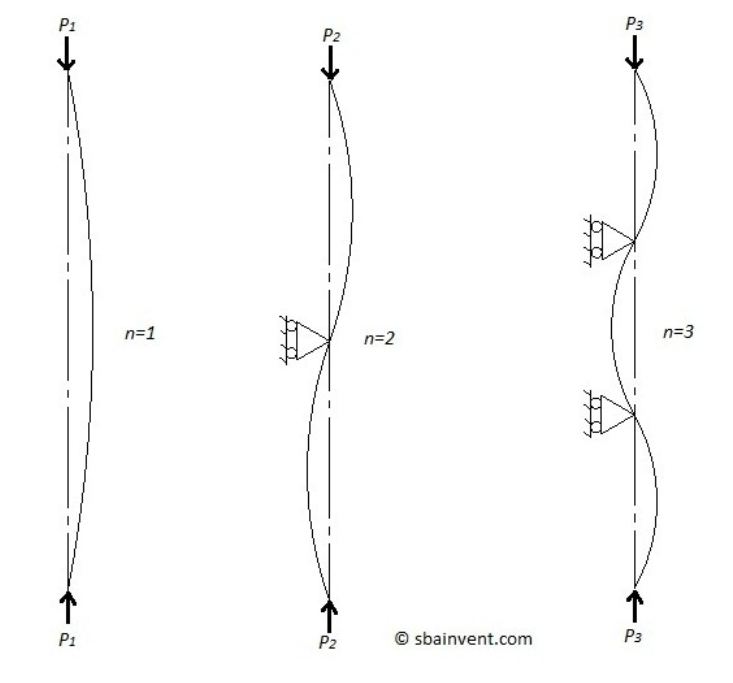
\includegraphics[scale=0.6, frame]{buckling2.png}
        \\Figure 3: Buckling with Various Numbers of Joints
    \end{center}

    \indent After unloading the truss, the members that experienced the second mode buckling also experienced plastic deformation, This is most likely because the cross-sectional area of the members were very small. When calculating the cross-sectional areas according to our targeted yield load, we were arriving at very small areas, that do not exist to be purchased because we used steel as our material, which has a yield strength of 36 ksi. We had to pick members based on the closest cross-sectional areas we could find. We also had to choose different members depending on whether or not the member was in tension or compression. In theory, each we could have had at least 3 different cross-sectional areas, one for the members in tension, of for the members in compression, and one for the zero-force members. This resembled the reality that full-scale bridges have many different types of members. In addition, under real loads, zero-force members usually do experience forces. Because of this, the zero-force members caused a slight deflection in the bottom chord of the truss. However, this deflection was elastic deformation and was minor compared to the buckling.  \\
    \indent During the fabrication of our bridge, we had to cut, clean, and connect our members. We chose steel for our design, and as a result, we were able to weld our bridge. Because the cross-sectional area of our members were small, we were able to use a hack saw to cut the members down. When cutting the members, we allowed for some of the material to be lost as a result of cutting. This is called kerf and is directly related to the width of the cut. In addition, all of the members had to be cleaned because steel is shipped with a protective oil coating to prevent rusting if the package gets wet during shipment. Not cleaning off this oil can cause issues while welding, especially when the electrode heats up the steel. While welding, the small cross-sectional areas of the members presented a challenge, where the ends of the rods were overheating and turning orange from getting too hot. In order to prevent this, we had to weld fast, creating small tack welds. In addition, we moved back and forth between the different ends of the truss, to allow the welds and members to cool down, before going back to an area near a hot weld. If the member becomes too hot and melts, this can change the physical properties of the steel, which could weaken its performance when tested. Lastly, we had to go over all of the welds, filling in all of the holes, and making sure the welds achieved full penetration - this means that the welds went completely through both sides of the member and that the welds were all around the joint. Because all of the load is applied at the joints of a truss, we had to make sure that there were no weak points in the welds, where the connection could possibly snap during loading. 

    \newpage
    \section{Conclusion}
    \indent The 6-foot truss bridge was designed to fail with 800 to 1000 pounds of idealized loading at the topmost joints: 400 pounds applied to each side truss. The design process considered the minimum cross-section required to take the load. The structure also had to resist buckling until a load of 800 pounds was reached; this required a larger cross section than a stress analysis determined. With buckling considerations, the bridge was designed such that it could take 502 pounds on each side truss. \\
    \indent The load testing itself found the bridge failing at 770.5 pounds of force, with second order buckling in the top chords on one end of the truss bridge. The bridge should have failed with the same behavior on each side of the bridge due to symmetry, if it were in fact centered under the hydraulic press unit. The asymmetric failure indicated that the bridge was not centered under the load; this was true observationally, despite efforts to ensure it was centrically placed. It is likely that if the bridge had been placed centrically, the bridge could have borne the actual design load and failed appropriately between 800 and 1000 pounds. \\
    \indent The members which experienced second order buckling also experienced plastic deformation; this is the failure that was designed for. Steel will experience elastic deformation until a yield point, after which deformation becomes plastic; for the purposes of this experiment, yield or plastic deformation was defined as failure, rather than rupture, because rupture is less able to be defined precisely. \\
    \indent The difference between the experimental and theoretical loads at which the bridge yielded is 233.5 pounds, giving a percent error of 23\%. The difference between required yield load and experimental yield load is only 29.5 pounds, carrying a percent error of 3.7\%. For the parameters of the assignment, the design performed very well, with small error. Error was larger when considering full design load capacity, but within reason considering the estimations and uncertainties involved in both design and testing conditions. \\
    \indent Error can be introduced in this experiment in many ways. Experimental and/or instrumental error can be introduced if the hydraulic press is improperly calibrated or leveled prior to testing; it is also possible for it to be introduced if the added plate used to distribute the load is not of known weight, which would lead to incorrect experimental load data. Procedural error can be introduced if the bridge is not precisely placed such that the loading occurs as was idealistically designed for; in this experiment, this is known to be a source of error. Further error can be introduced during the welding process; if the steel reached temperatures such that the material composition changed slightly, the bridge would not behave as intended, due to inconsistencies in the metal that cannot be truly accounted for. Further, if some joints are welded poorly and cannot carry load, this would impact the bridge's overall ability to take weight. Error in calculations can be introduced during the iterative processed used to determine the steel cross-section of the bridge members, due to rounding, or in reading the force-deflection curve created during loading, which would result in an incorrect experimental load value or deflection. Other possible calculation errors can be in the choice of a length factor in determining buckling; the precise \(k\) value was not known, since connections were welded and thus fixed rather than pinned but also cannot be assumed to be perfectly fixed. A factor of 0.83 was chosen as an option between the recommended design values for fixed-fixed and pinned-fixed connections; were the true \(k\) value known, it is possible a different cross section would have been the better choice.\\ 
    \indent Improvements on the experiment would serve the results well. It would be advisable to check placement more precisely, fix the distribution plate to the press, and have better, more stable placement of the supports under the bridge. 


    \newpage
    \section{References}
    \begin{enumerate}
        \item Ferdinand B. \emph{et. al.} (2015). \emph{Mechanics of Materials}, 7th Ed., McGraw Hill, New York.
        \item Seán C. (2020). Column Buckling Equations, \url{https://www.degreetutors.com/column-buckling-equations/} (accessed 5 October 2022).
        \item Russel H. (2017). \emph{Structural Analysis}, 10th Ed., Pearson, London.
    \end{enumerate}
    \newpage
    \section{Appendix}
    \addcontentsline{toc}{subsection}{Materials Pricing}

    % Cost Breakdown

    \addcontentsline{lot}{table}{Table 1: Materials Pricing}
    {\centering \large{\bf Table 1: Materials Pricing\\}}
    \begin{center}
        \begin{tabular}{|l|l|l|l|}
            \hline
            \textbf{Item} & \textbf{Unit Price} & \textbf{Quantity} & \textbf{Total Cost} \\\hline
            3/8" diameter HR CQ Steel Round - 8 ft & \$9.24 & 7 & \$64.68\\\hline 
            3/8" diameter HR CQ Steel Round - 6 ft & \$7.18 & 2 & \$14.36\\\hline 
            3/16" diameter HR CQ Steel Round - 6 ft & \$7.72 & 2 & \$15.44\\\hline
        \end{tabular}
        \vspace{10mm}

        % Information for Materials Suppliers

        {\large{\bf Materials Supplier\\}}
        \vspace{3mm}
        Metals Depot International\\
        4200 Revilo Road\\
        Winchester, KY 40391\\
        1-859-745-2650\\
    \end{center}
    \newpage

    % Robot Data

    \addcontentsline{toc}{subsection}{Finite Element Analysis}
    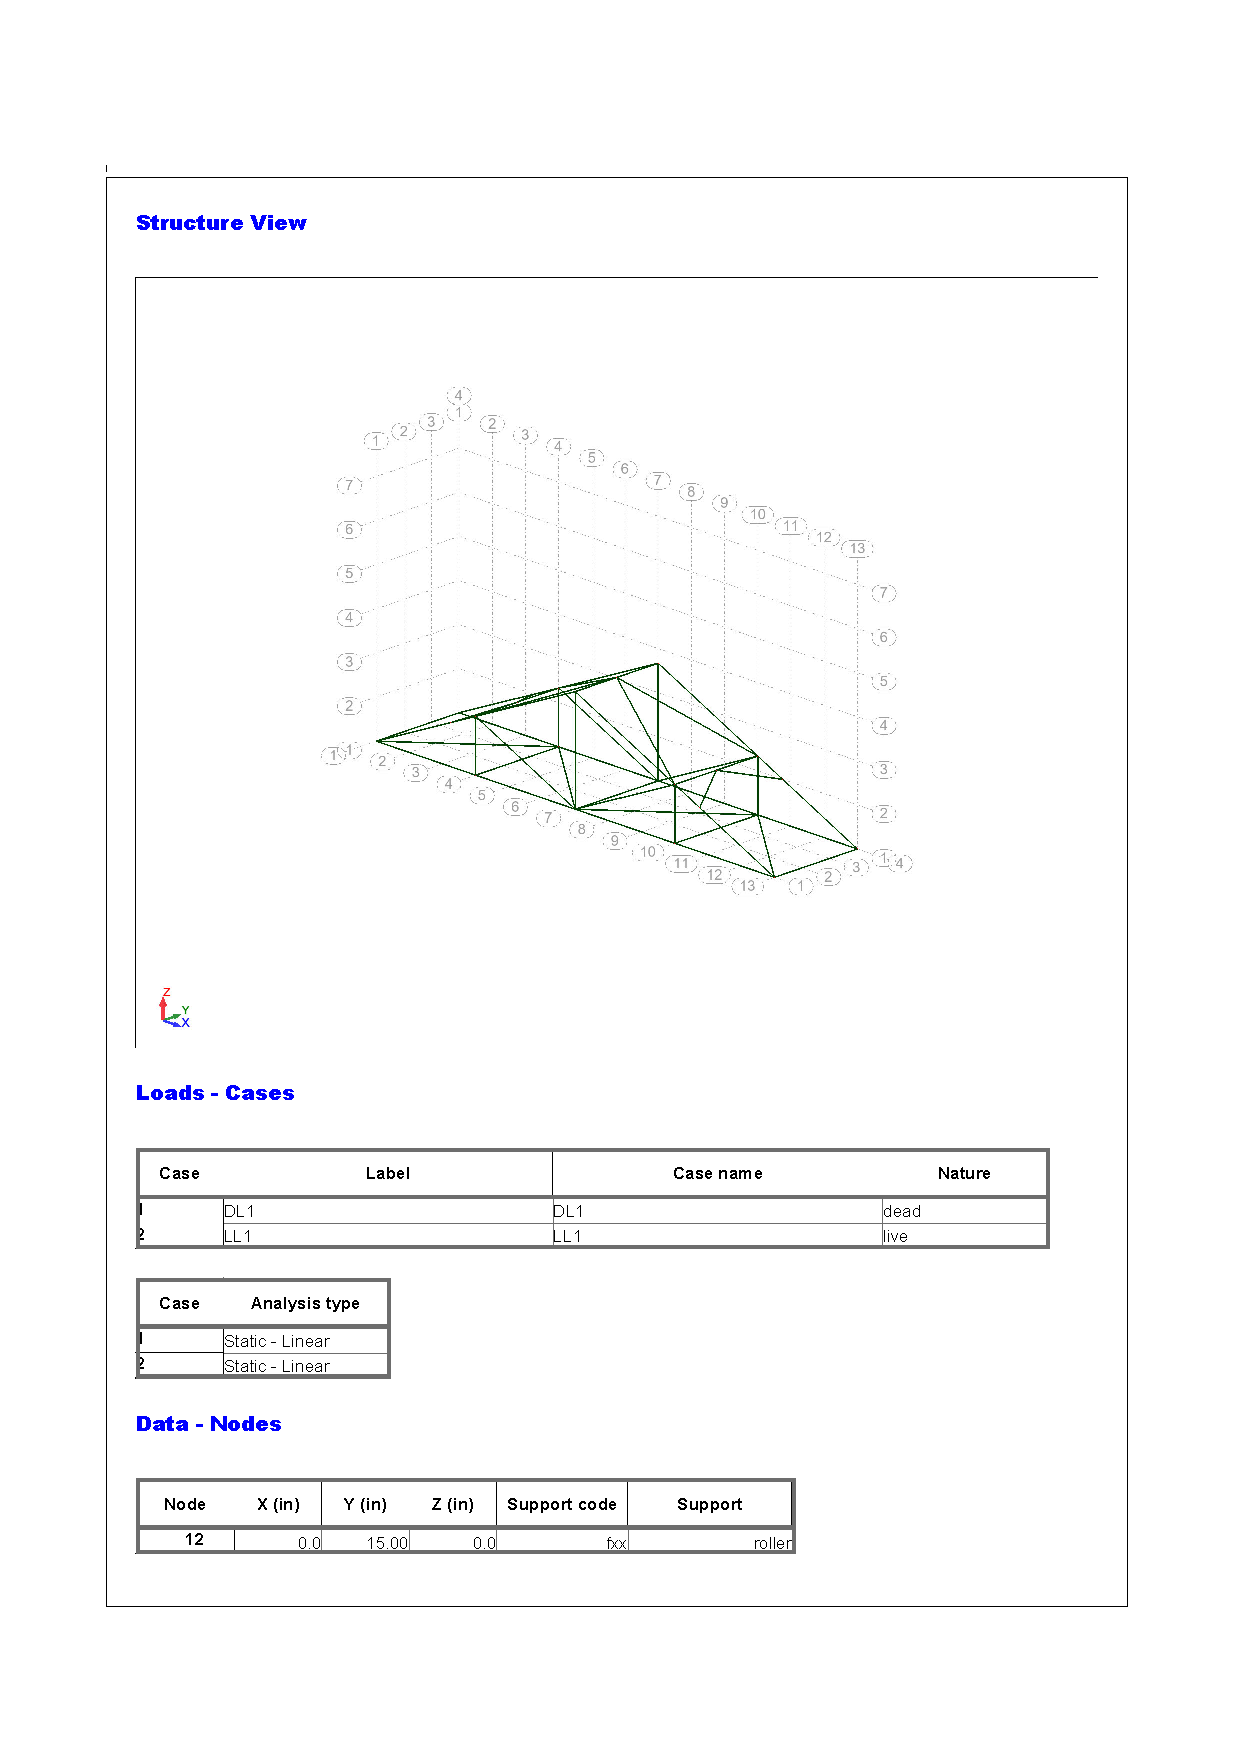
\includepdf[pages=-,pagecommand={\phantomsection\thispagestyle{fancy}}]{bridge robot data.pdf}
    \newpage

    % Connections
    \begin{landscape}
    \addcontentsline{toc}{subsection}{Connection Drawings}
    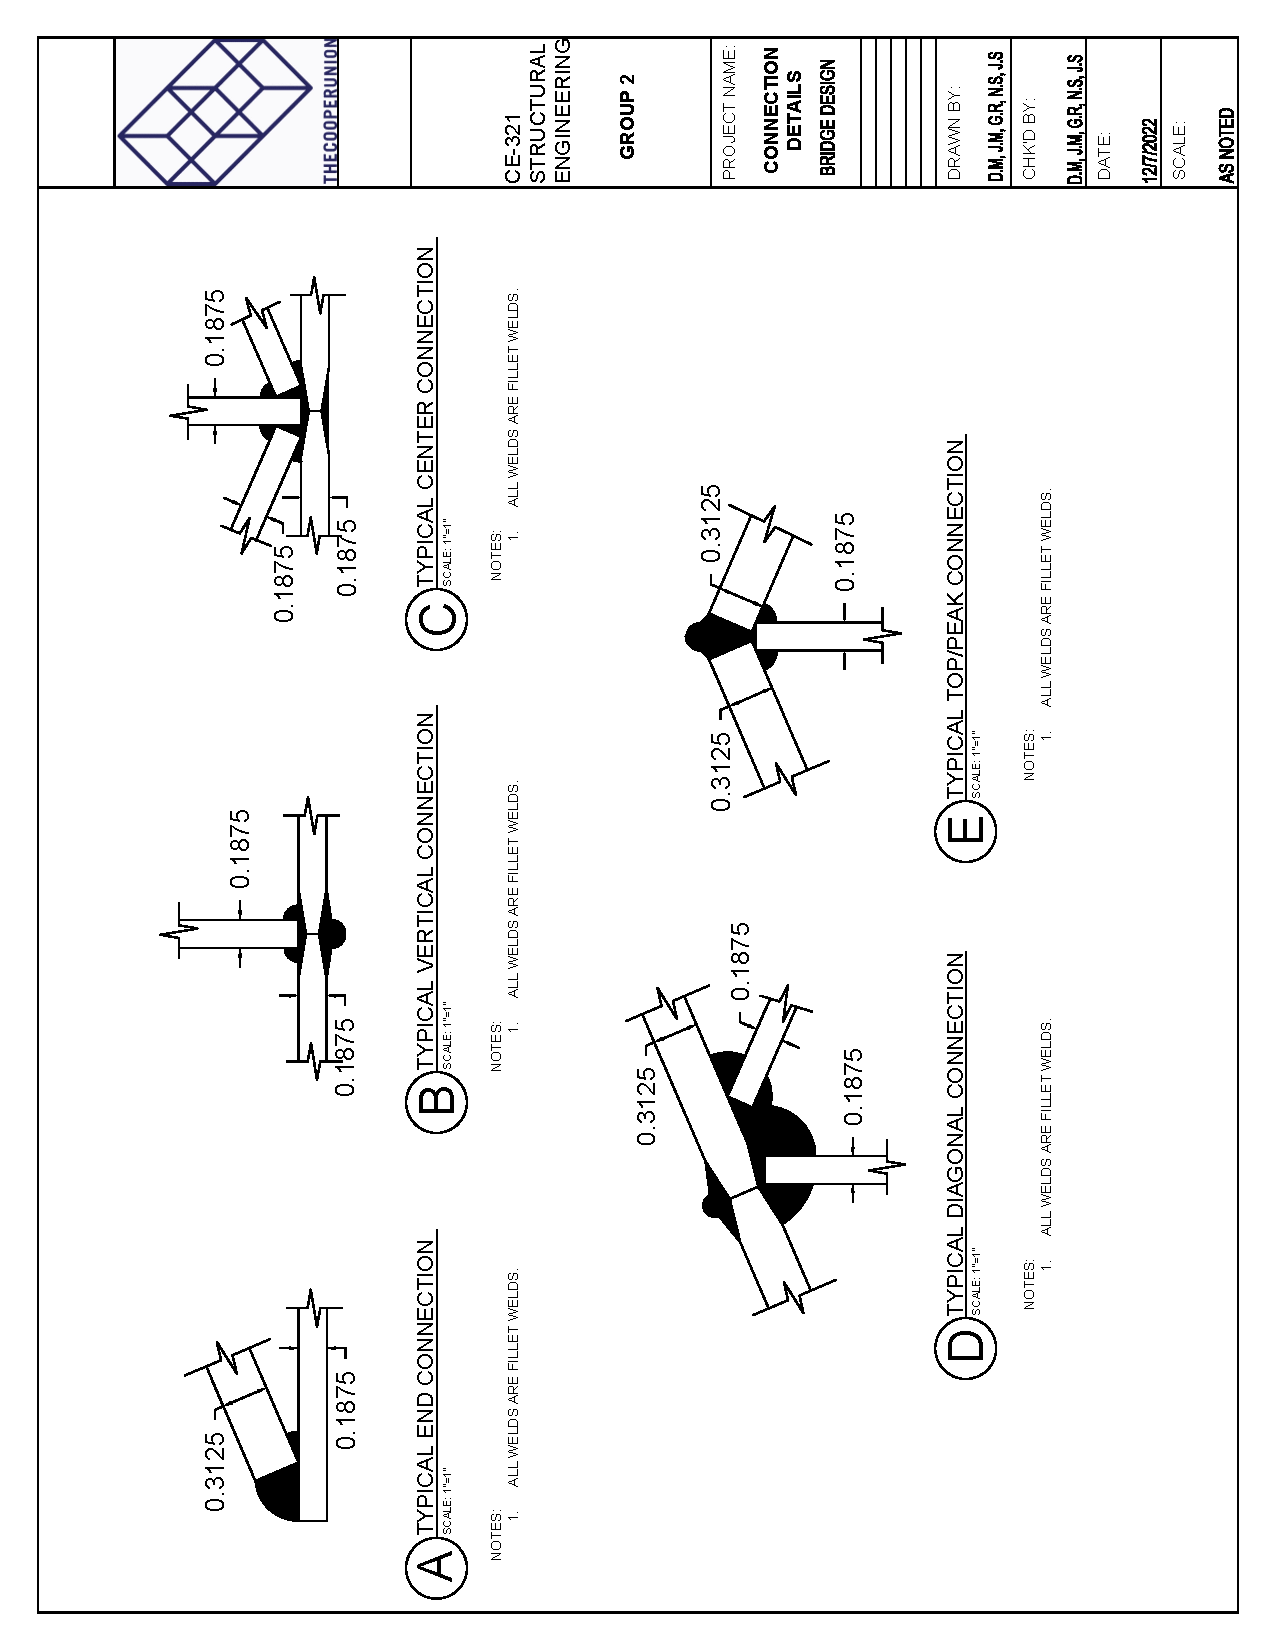
\includepdf[pages=-,pagecommand={\phantomsection\thispagestyle{empty}}]{connections.pdf}
    \end{landscape}
    \newpage

    % All 2D Drawings
    \begin{landscape}
    \addcontentsline{toc}{subsection}{Initial Design - David Madrigal}
    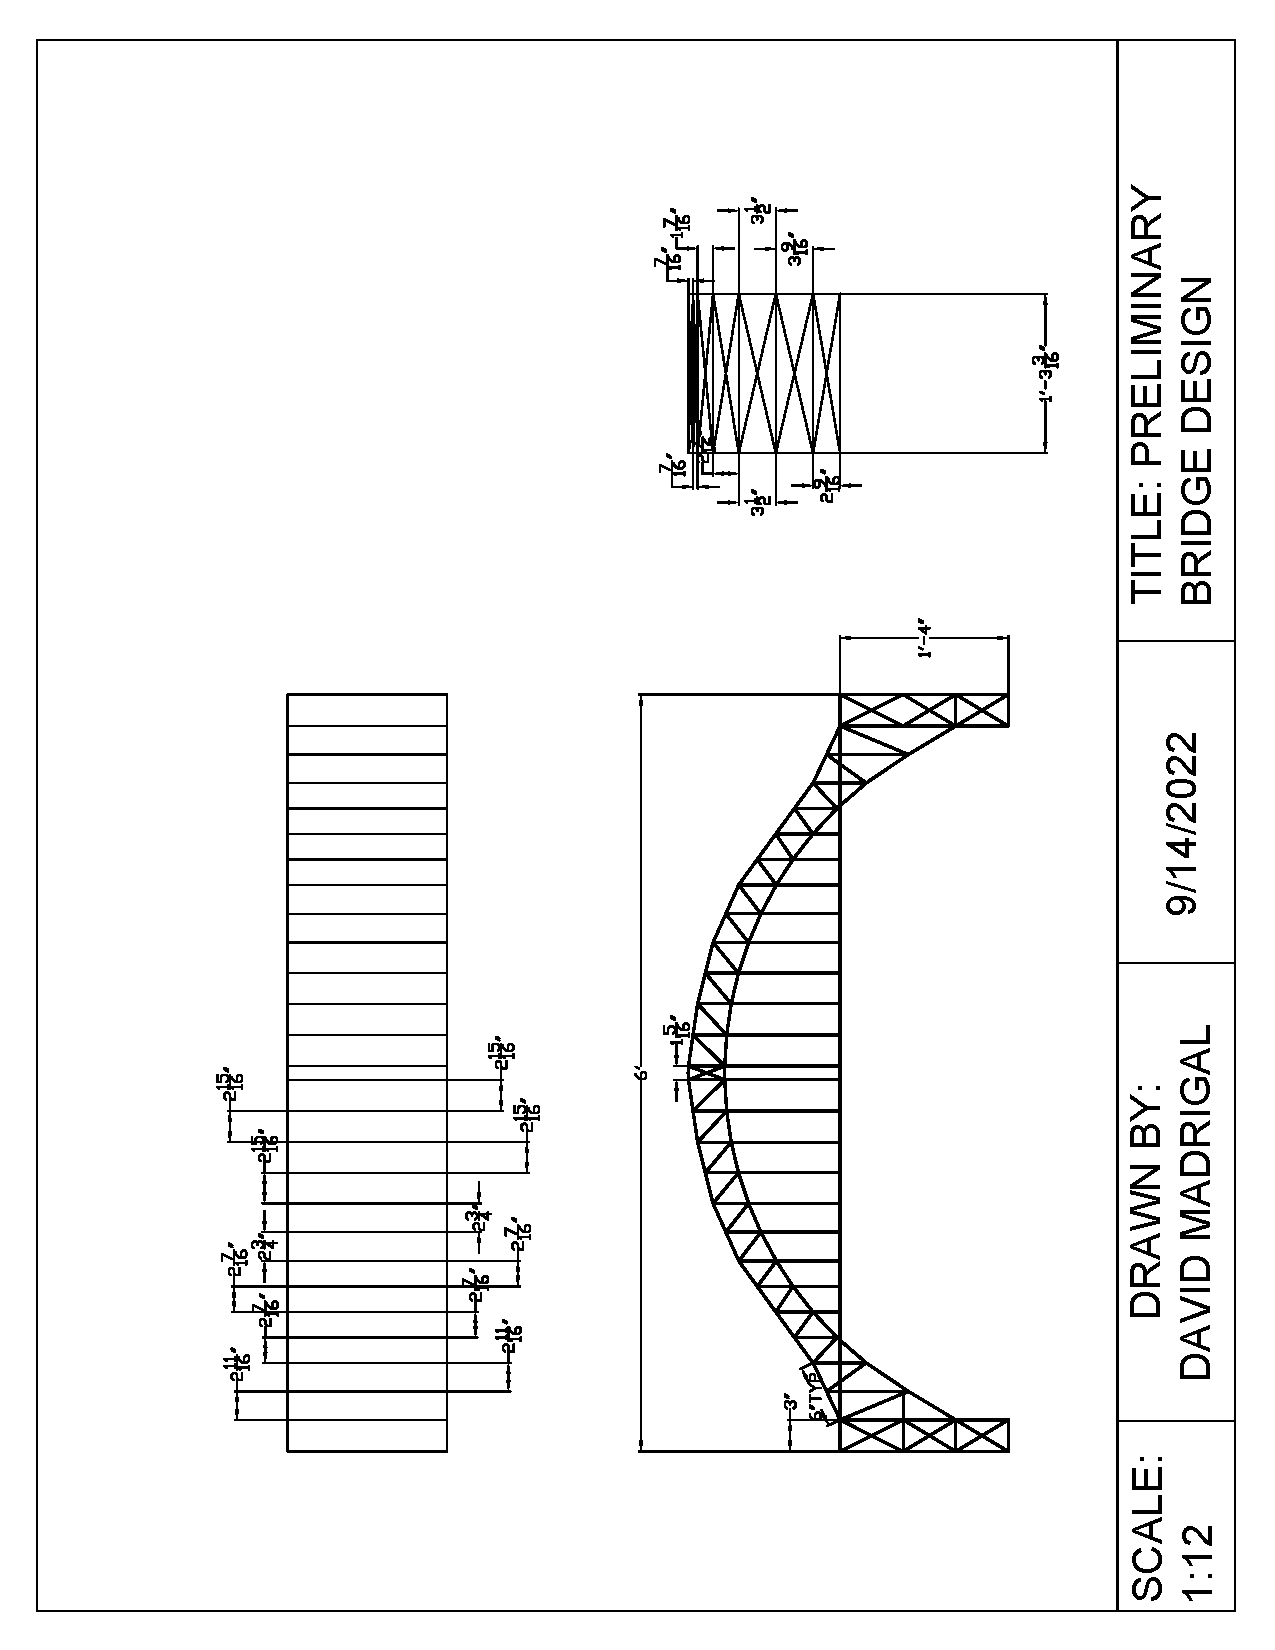
\includepdf[pages=-,pagecommand={\phantomsection\thispagestyle{empty}}]{dm.pdf}
    \end{landscape}
    \newpage
    
    \begin{landscape}
    \addcontentsline{toc}{subsection}{Initial Design - Jenna Manfredi}
    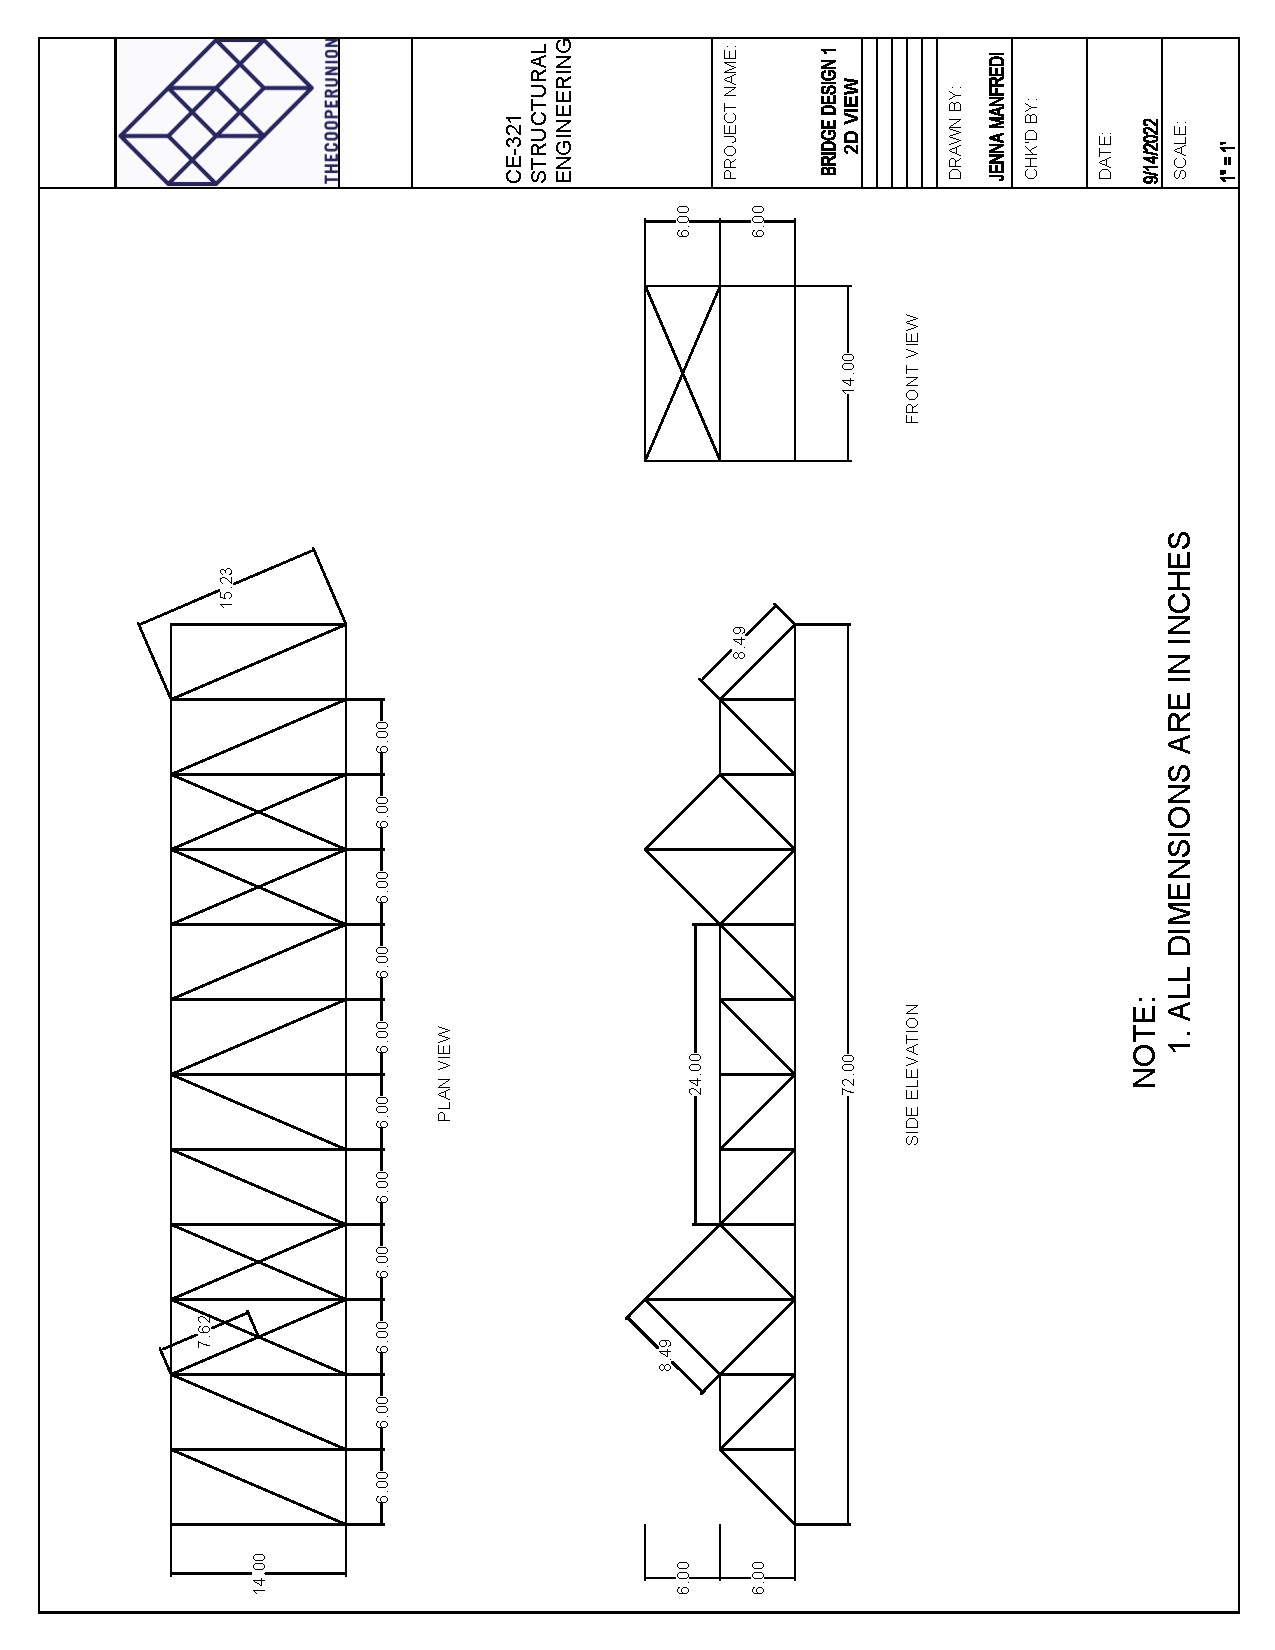
\includepdf[pages=-,pagecommand={\phantomsection\thispagestyle{empty}}]{jm.pdf}
    \end{landscape}
    \newpage

    \begin{landscape}
    \addcontentsline{toc}{subsection}{Initial Design - Jacob Sigman}
    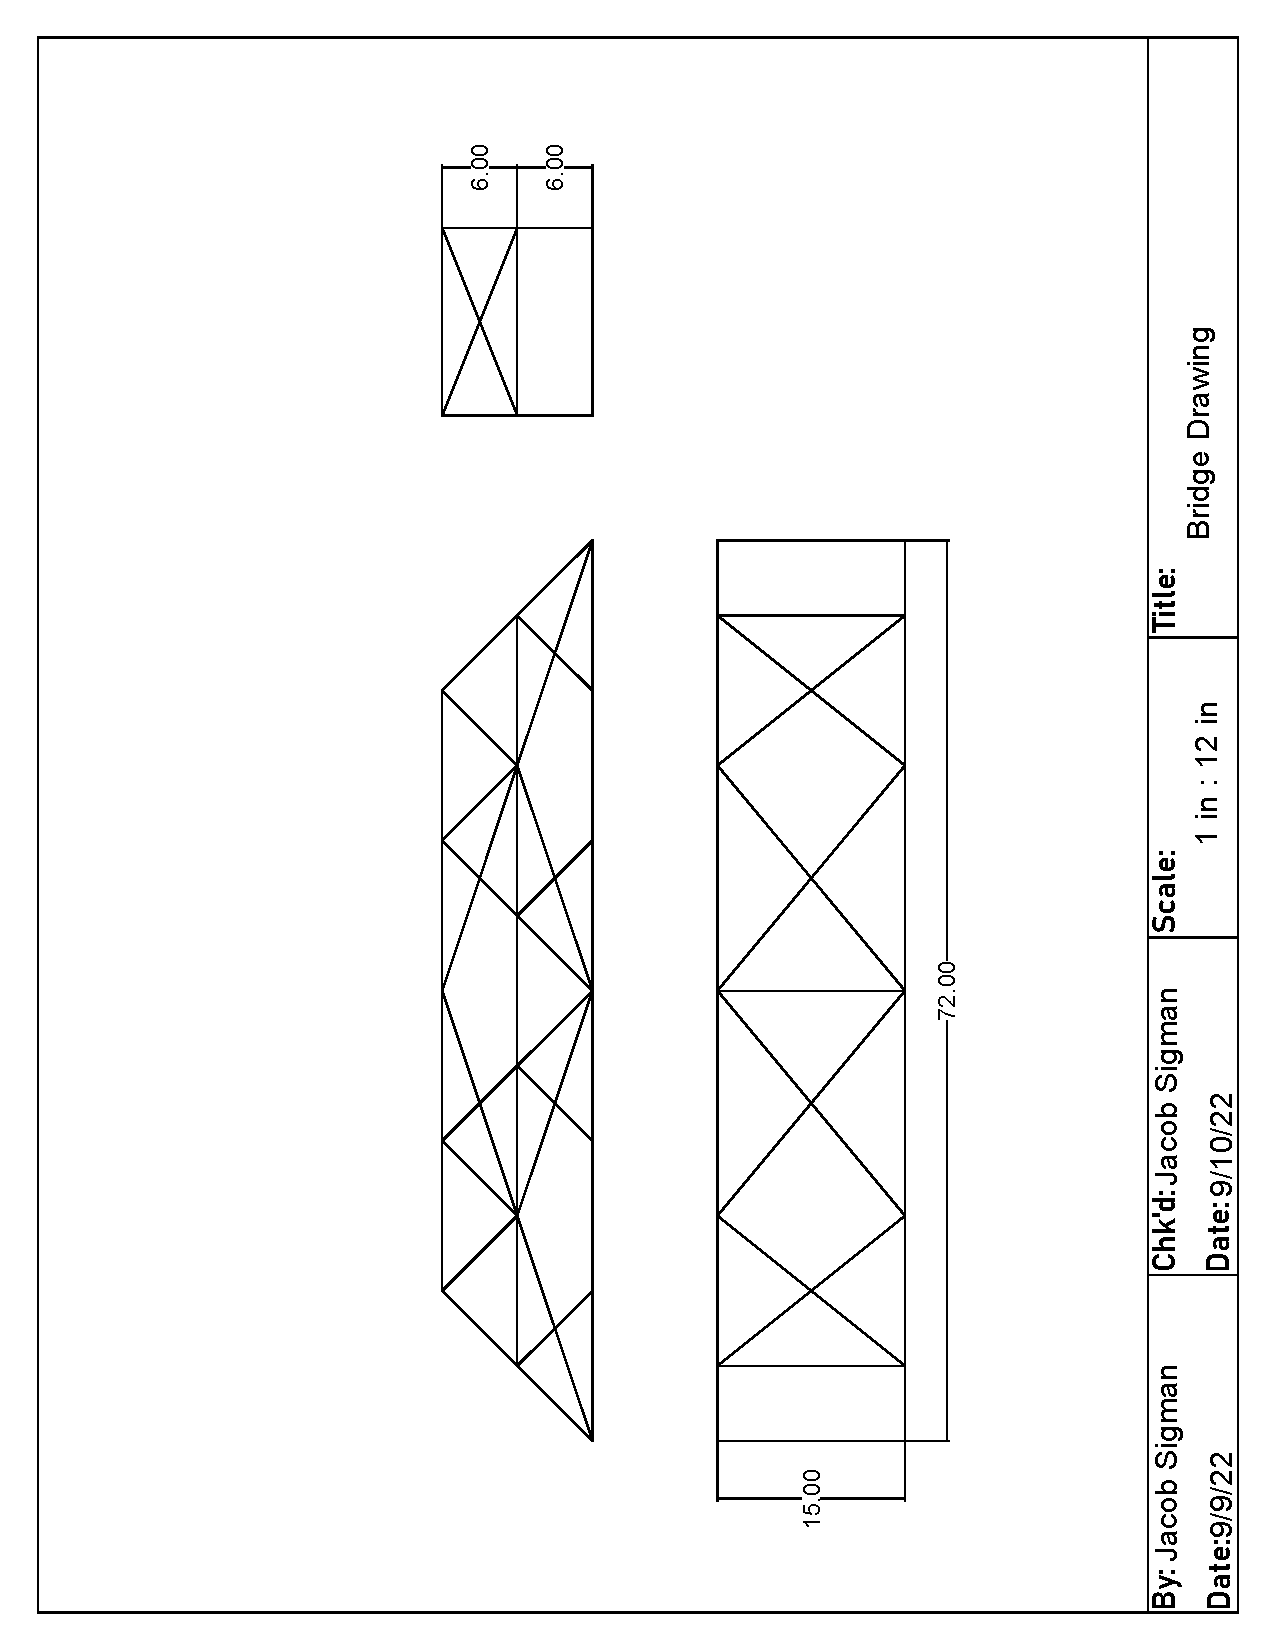
\includepdf[pages=-,pagecommand={\phantomsection\thispagestyle{empty}}]{js.pdf}
    \end{landscape}
    \newpage

    \begin{landscape}
    \addcontentsline{toc}{subsection}{Initial Design - Nicole Shamayev}
    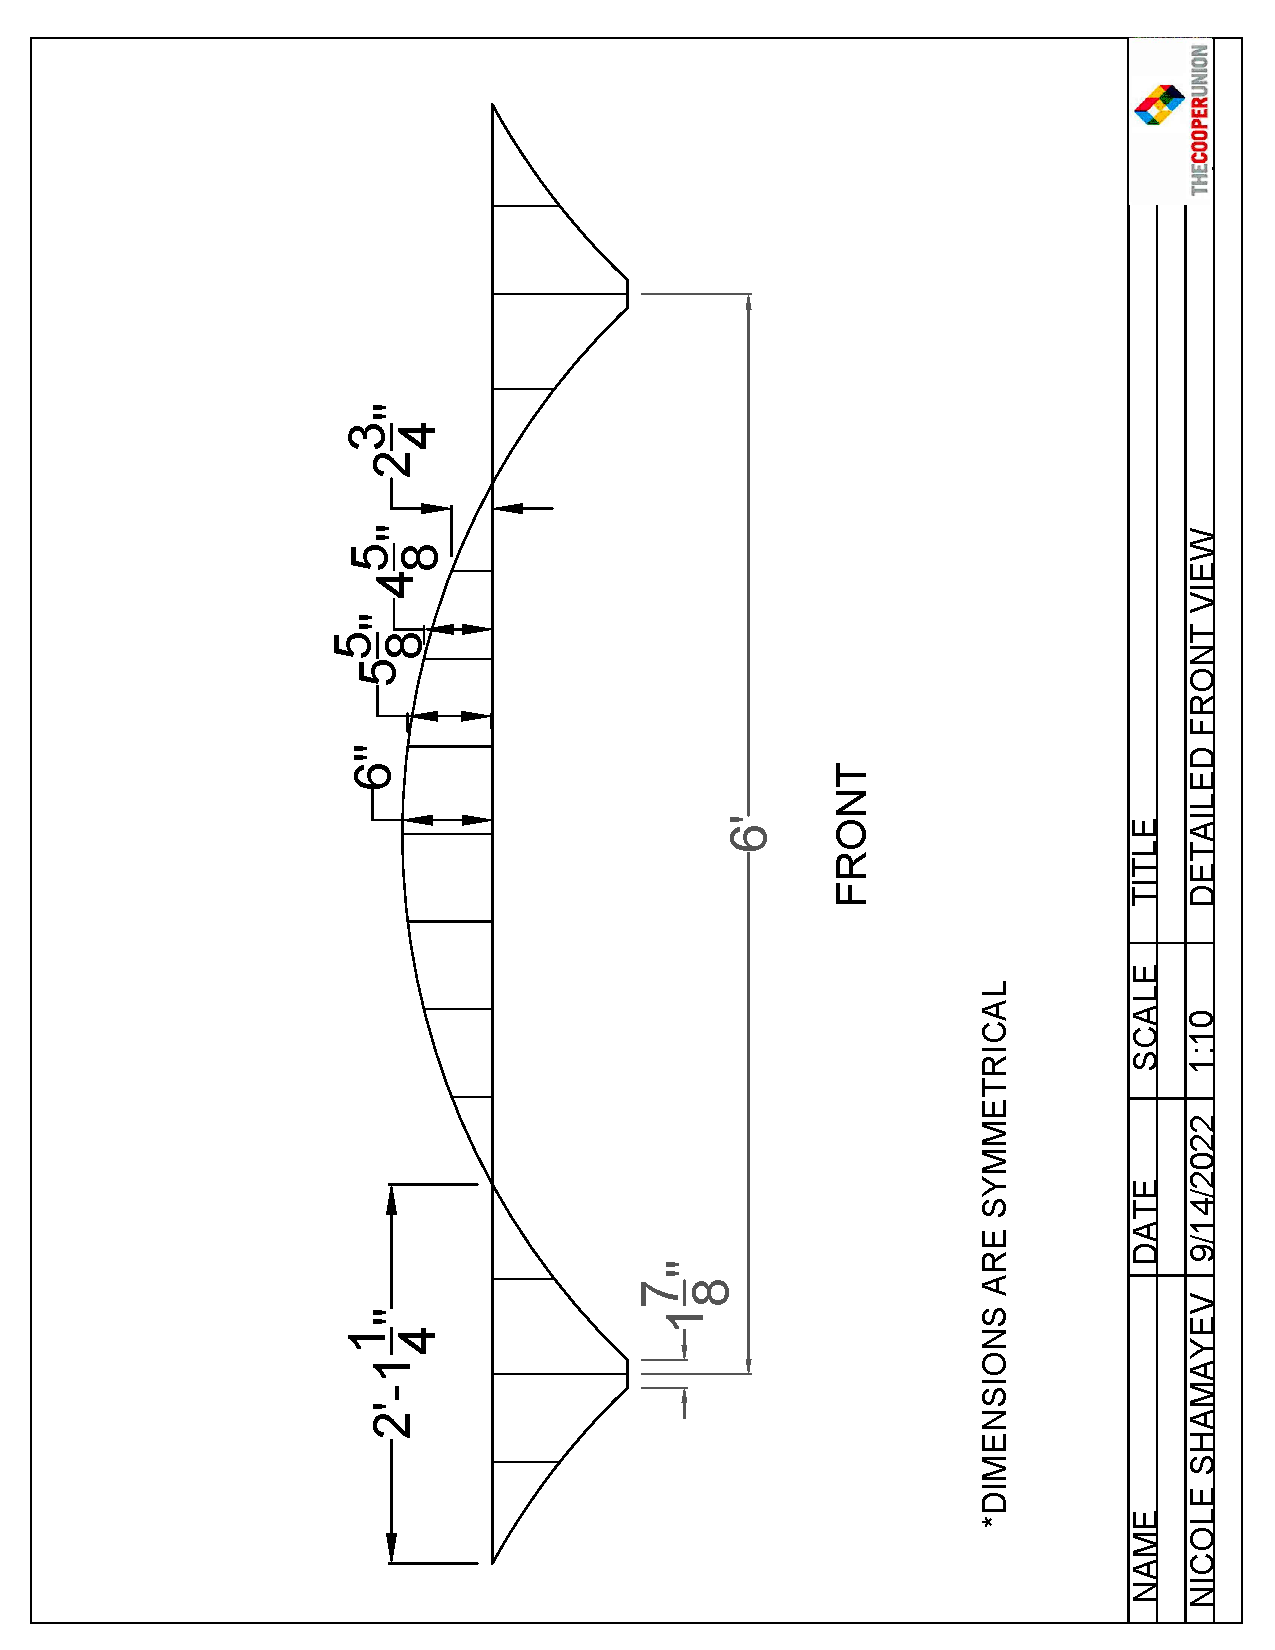
\includepdf[pages=-,pagecommand={\phantomsection\thispagestyle{empty}}]{ns.pdf}
    \end{landscape}
    \newpage

    \begin{landscape}
    \addcontentsline{toc}{subsection}{Initial Design - Gila Rosenzweig}
    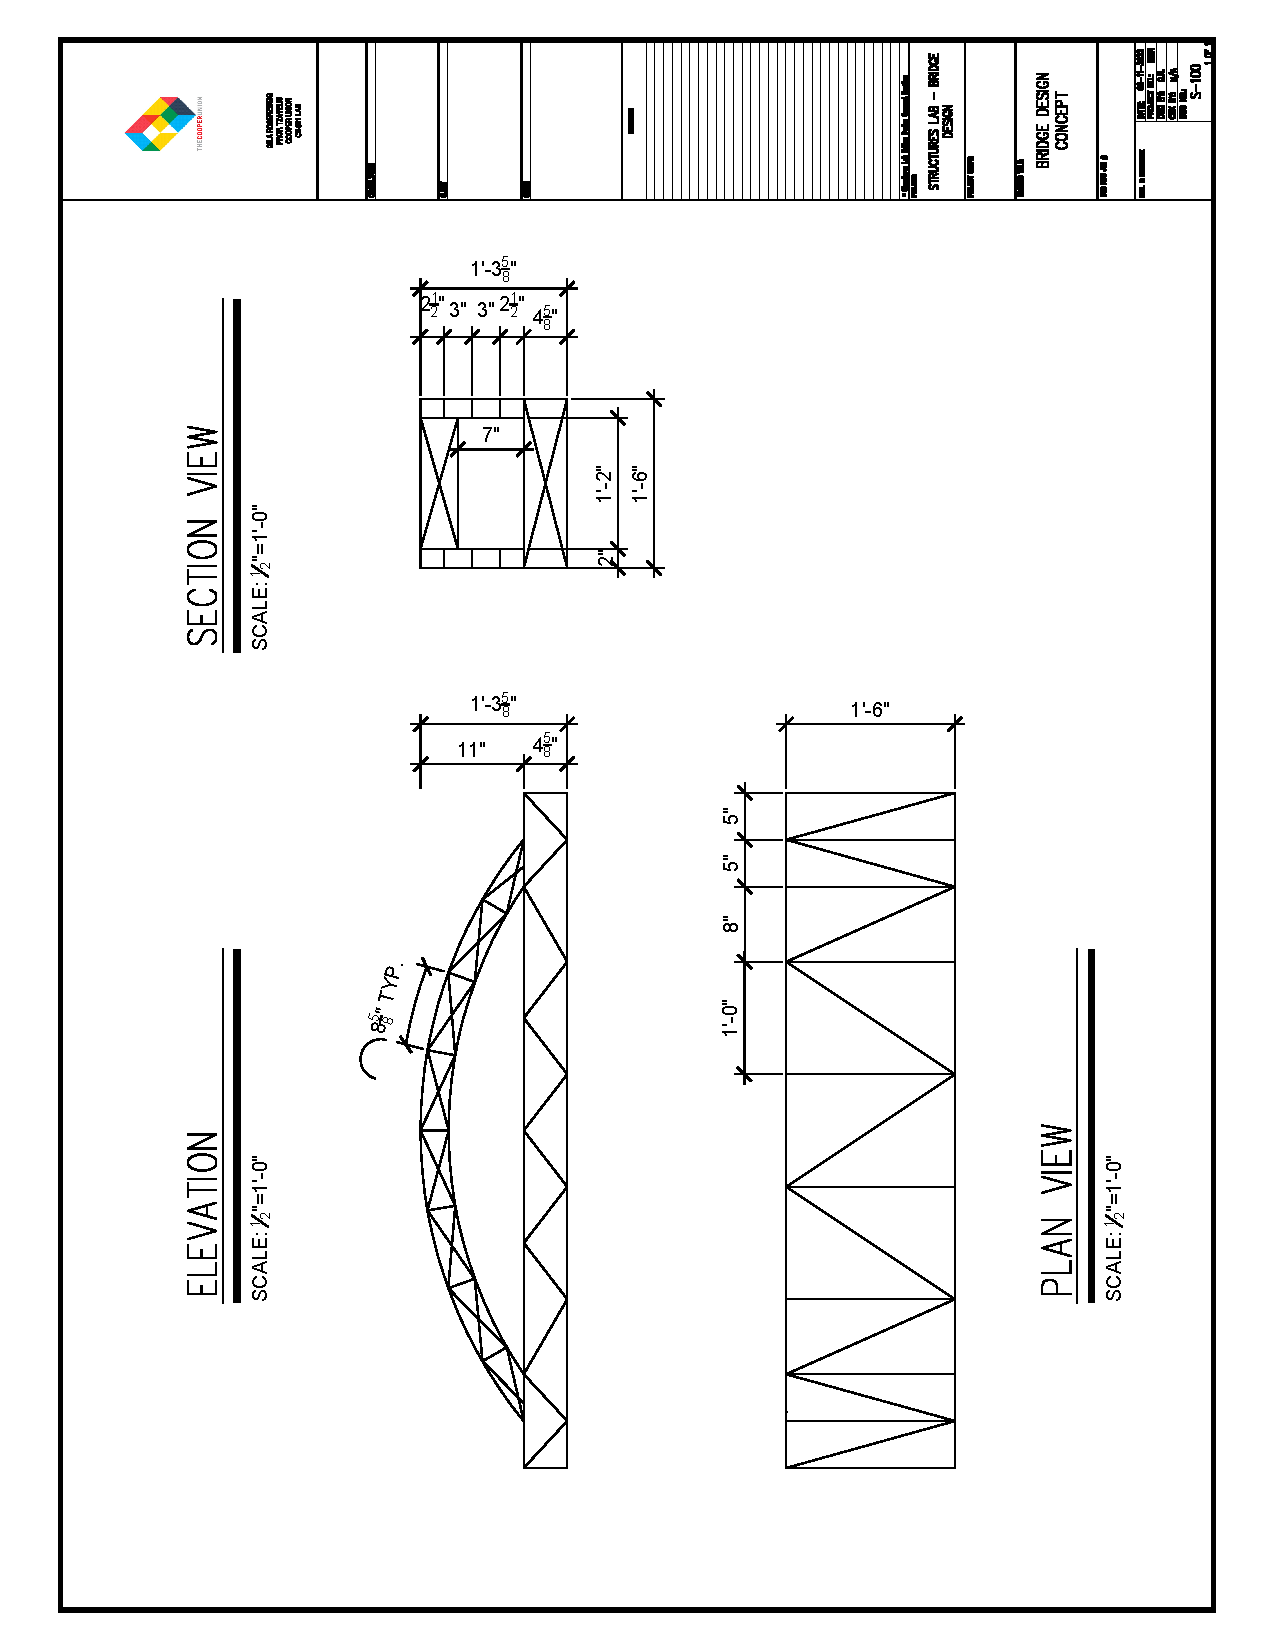
\includepdf[pages=-,pagecommand={\phantomsection\thispagestyle{empty}}]{gr.pdf}
    \end{landscape}
    \newpage
   

    
\end{document}